% Cal Poly Thesis
% 
% based on UC Thesis format
%
% modified by Mark Barry 2/07.
%

\documentclass[12pt]{ucthesis}
\usepackage{ifpdf}

\let\ifpdf\relax

\newif\ifpdf
\ifx\pdfoutput\undefined
    \pdffalse % we are not running PDFLaTeX
\else
\pdfoutput=1 % we are running PDFLaTeX
\pdftrue \fi

\usepackage{url}
\ifpdf

    \usepackage[pdftex]{graphicx}
    % Update title and author below...
    \usepackage[pdftex,plainpages=false,breaklinks=true,colorlinks=true,urlcolor=blue,citecolor=blue,%
                                       linkcolor=blue,bookmarks=true,bookmarksopen=true,%
                                       bookmarksopenlevel=3,pdfstartview=FitV,
                                       pdfauthor={Joseph White},
                                       pdftitle={PARIS: A PArallel RSA-prime InSpection tool},
                                       pdfkeywords={thesis, masters, cal poly}
                                       ]{hyperref}
    %Options with pdfstartview are FitV, FitB and FitH
    \pdfcompresslevel=1

\else
    \usepackage{graphicx}
\fi

\usepackage{amssymb}
\usepackage{amsmath}
\usepackage[letterpaper]{geometry}
\usepackage[overload]{textcase}
\usepackage{url}
\usepackage{array}

\setlength{\parindent}{0.25in} \setlength{\parskip}{6pt}

\geometry{verbose,nohead,tmargin=1.25in,bmargin=1in,lmargin=1.5in,rmargin=1.3in}

\setcounter{tocdepth}{2}

% Different font in captions (single-spaced, bold) ------------
\newcommand{\captionfonts}{\small\bf\ssp}
% ---------------------------------------

\begin{document}

\title{PARIS: A PArallel RSA-prime InSpection tool}
\author{Joseph White}
\degreemonth{June} \degreeyear{2013} \degree{Master of Science}
\defensemonth{May} \defenseyear{2013}
\numberofmembers{3} \chair{Chris Lupo, Ph.D.} \othermemberA{Phillip Nico, Ph.D.} \othermemberB{Foaad Khosmood, Ph.D.}
\field{Computer Science} \campus{San Luis Obispo}
\maketitle

\begin{frontmatter}
% Custom made for Cal Poly (by Mark Barry, modified by Andrew Tsui).
\copyrightpage
% Custom made for Cal Poly (by Andrew Tsui).
\committeemembershippage


\begin{abstract}

Modern-day computer security relies heavily on cryptography as a means to
protect the data that we have become increasingly reliant on. As the Internet
becomes more ubiquitous, methods of security must be better than ever.
Validation tools can be leveraged to help increase our confidence and
accountability for methods we employ to secure our systems. 

Security validation, however, can be difficult and time-consuming. As our
computational ability increases, calculations that were once considered ``hard"
due to length of computation, can now be done in minutes. We are constantly
increasing the size of our keys and attempting to make computations harder to
protect our information. This increase in ``cracking" difficulty often has the
unfortunate side-effect of making validation equally as difficult.

We can leverage massive-parallelism and the computational power that is granted
by today's commodity hardware such as GPUs to make checks that would
otherwise be impossible to perform, attainable. Our work presents a practical tool for
validating RSA keys for poor prime numbers: a fundamental problem that has led
to significant security holes.

Our implementation using NVIDIA's CUDA framework offers a 27.5 times speedup
over a reference sequential implementation. This level of speedup brings this
validation into the realm of runtime reachability.


\end{abstract}


\tableofcontents


\listoftables
\listoffigures
\end{frontmatter}


\pagestyle{plain}
\renewcommand{\baselinestretch}{1.66}

% ------------- Main chapters here --------------------

\chapter{Introduction}
\label{introduction}

%%%%%%%%%%%%%%%%%%%%%%%%%%%%%%%%%%%%%%%%%%%%%%%%%%%%%%%%%%%%%%%%%%%%%%%%%%%%%%%

\chapter{Background}
\label{background}
RSA is an asymmetric key encryption scheme. Keys come in matched pairs:
public keys and private keys. Using the same algorithm, information encrypted
with the one key, can be decrypted with the other and vice versa. A party must
keep the private keep secret, but the public portion of the key can be seen and
used by anyone in the world. To generate a pair, an algorithm is performed on
two randomly-generated prime numbers whose product is of a certain bit-length
(e.g. 1024 bits). These are the primes that our work looks to discover
inadequacies with.

The work presented by Lenstra et. al. \cite{lenstra2012ron} shows that around
0.2\% of RSA keys collected from sources including the SSL Observatory suffer
from inadequate random prime generation. They show that when the primes used to
build an RSA public-private key pair are not actually random, factoring does
not need to be done to break the keys. Instead, only a greater common divisor
needs to be calculated between two RSA moduli. When anything greater than 1 is
found as a result of this calculation, the keys can be considered broken and
offer no protection. This is because once a GCD greater than 1 is found, the
private keys can be generated from the publicly available information. The
vulnerability is explained in detail in Figure \ref{fig:vuln}.

\begin{figure}
   \centering
   \includegraphics[width=\linewidth]{vulnerability.png}
   \caption{Explanation of poor-prime vulnerability}
   \label{fig:vuln}
\end{figure}

A tool by Scharfglass et. al. \cite{scharfglass2012breaking} performs a
parallelized version of this GCD calculation (using the binary GCD algorithm)
between every pair combination in a given set of keys. It structures these
calculations so that as many as possible can be done at once. To increase
parallelism, and because the keys are so large, they are broken up into 32
chunks, which are also operated on in parallel using the GPU. Through these 2
levels of parallelism, a speedup of 27.5 is achieved. This tool provides a
practical tool for checking a given set of keys for the vulnerability we are
focusing on.

\section{Motivation}
Scharfglass et. al. use NVIDIA's CUDA framework to significantly speedup a check for the vulnerability
presented in \cite{lenstra2012ron}. The work in \cite{scharfglass2012breaking}
lacks any context or explanation of usage for RSA keys in general, and although
their data set is security- and encryption-focused, no discussion is given to
the security aspects and the potential impacts of the work. Some research was
done in an attempt to add context to the work, and the implications it might
have.

Most initial research yielded general statements that did not explain or give
appropriate context to RSA (statements including ``\dots all over the
Internet\dots" were accurate, but not informative). More in-depth research
yielded two primary use-cases of RSA: Digital Rights Management (DRM) and
Secure Socket Layer (SSL) and Transport Layer Security (TLS) Internet
security protocols. Other uses included password alternatives (e.g. ssh
connections or command line interface tools like \texttt{git}) but these are
more difficult to collect data for and analyze since they tend to be done on
an individual basis, and are managed by individual users.

\subsection{Digital Rights Management}
Digital rights management is a protocol used to secure the usage and
distribution of various types of media content. It is adopted by content
providers and device manufacturers to ensure users don't misuse or wrongfully 
share protected, copyrighted content.
The RSA Association proposed a protocol that could be applied to various types
of media content that secured its usage \cite{rsa2004announces,
rsa2004supports}. These announcements argued that using RSA for DRM offered
benefits to the content providers, the device manufacturers, and, arguably, the
consumers of the content. It apparently allowed device manufactures and
content providers to ensure proper usage of protected content while allowing
users to consume and playback their rightfully-owned media on an array of
their own devices.

\subsection{Internet Security and Certificates}
Internet security relies on a particular protocol called SSL and its successor
TLS. These protocols define how to securely transfer information over the
Internet by using encryption and signing mechanisms. One aspect of both the SSL
and TLS protocols involve certificates to ensure the expected party is
actually being communicated with. These certificates provide information
about a server that a user is connected to (e.g. Amazon or Google)
and is signed by a certificate authority (e.g. VeriSign). These certificates
are also encrypted with a subject's (e.g. Amazon) public key to ensure that
the entity is who they say they are. Furthermore, the public key is then used 
to transfer information back to the subject in a secure way. Figure
\ref{fig:tls} describes the TLS process between a client and server. 

The most widely used type of certificate is the X.509 certificate, whose current
revision is 3. A breakdown of the major sections of the certificate is shown in
Figure \ref{fig:x509}. The ``Subject Public Key Information" section of the
certificate holds the relevant data (the subject's RSA public key) for our work.
The public key portion of the certificates can actually use one of several
algorithms defined in the specification. RSA is by far the most popular,
accounting for over half of the found certificates (as shown in Figure
\ref{fig:certs}). Other options include DSA and Diffie-Hellman. For more
detailed information about X.509 certificates and analysis on their
infrastructure, see \cite{holz2011ssl}.

\begin{figure}
   \centering
   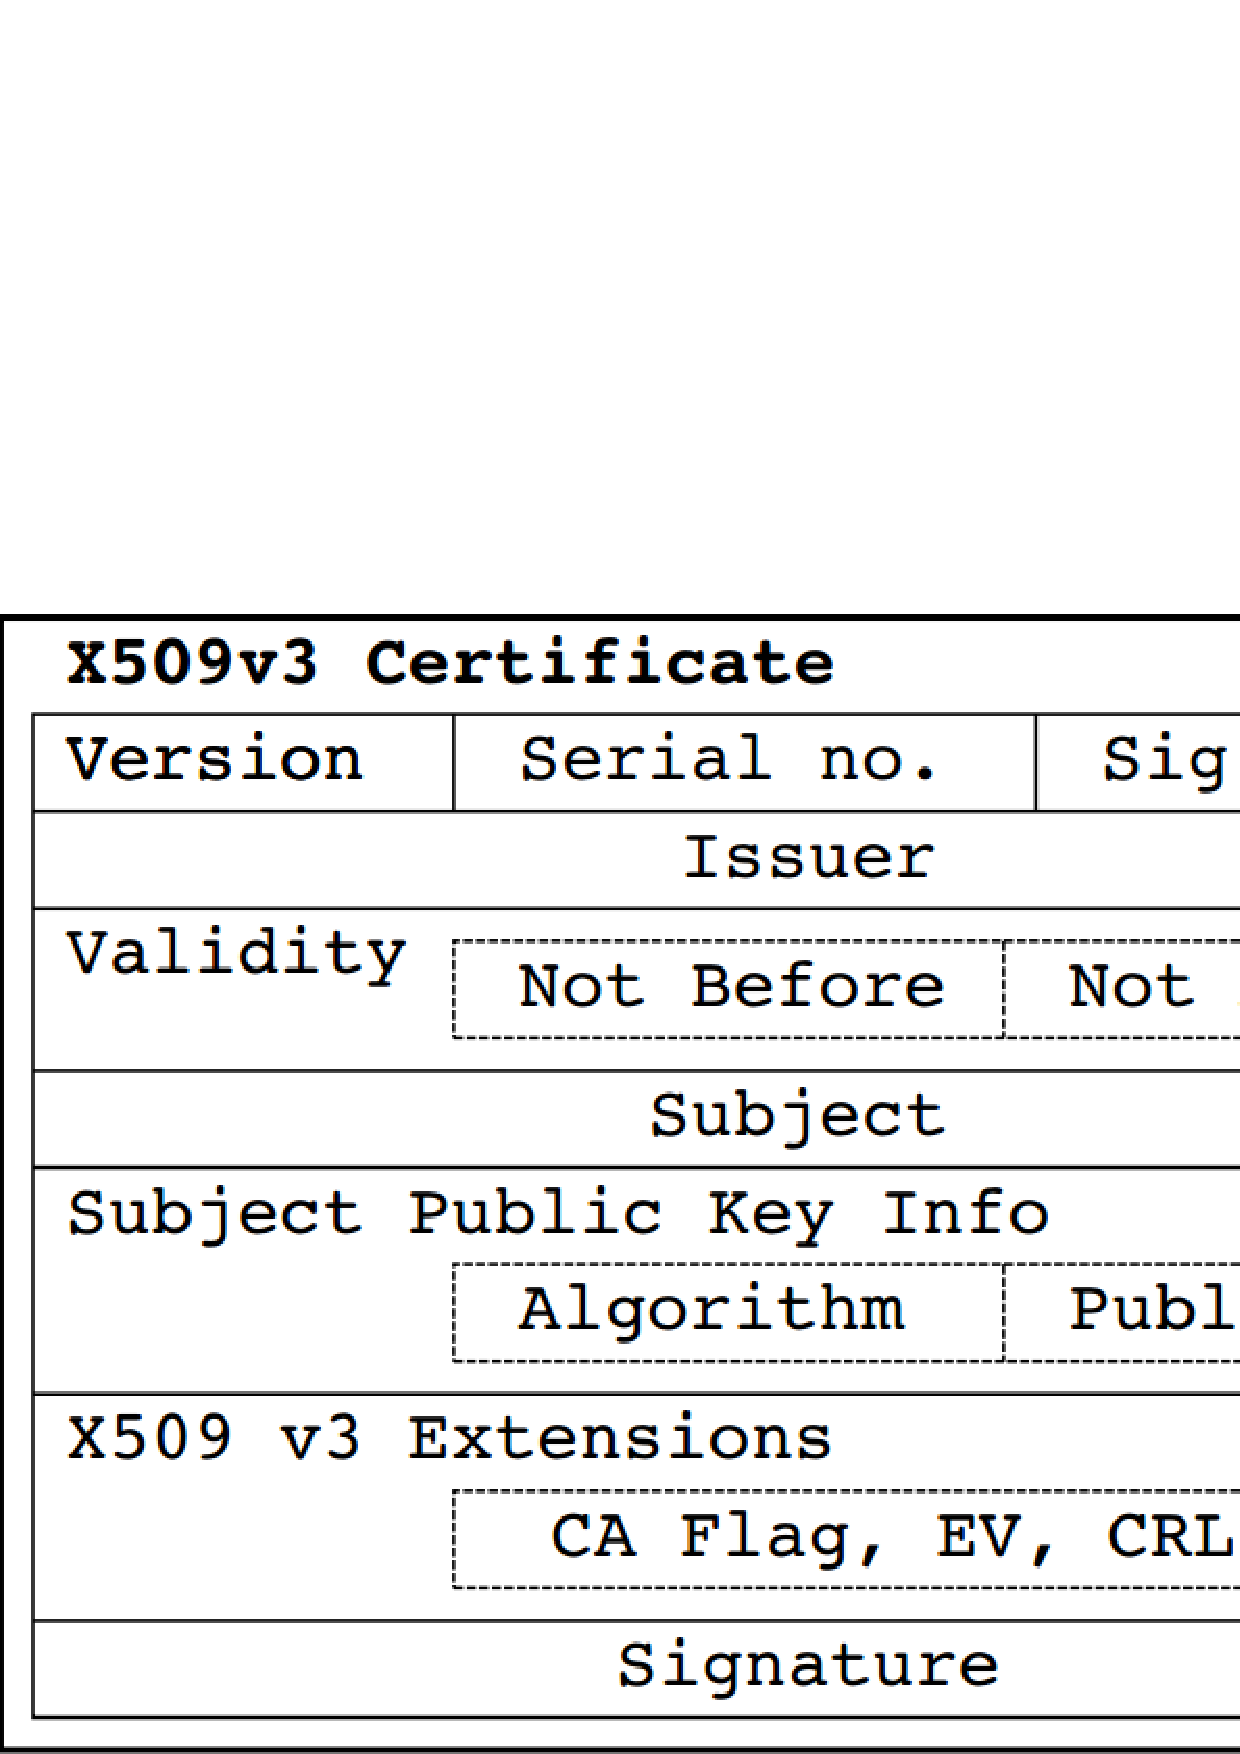
\includegraphics[width=0.5\linewidth]{x509.png}
   \caption{X.509 Fields\cite{holz2011ssl}}
   \label{fig:x509}
\end{figure}

\begin{figure}
   \centering
   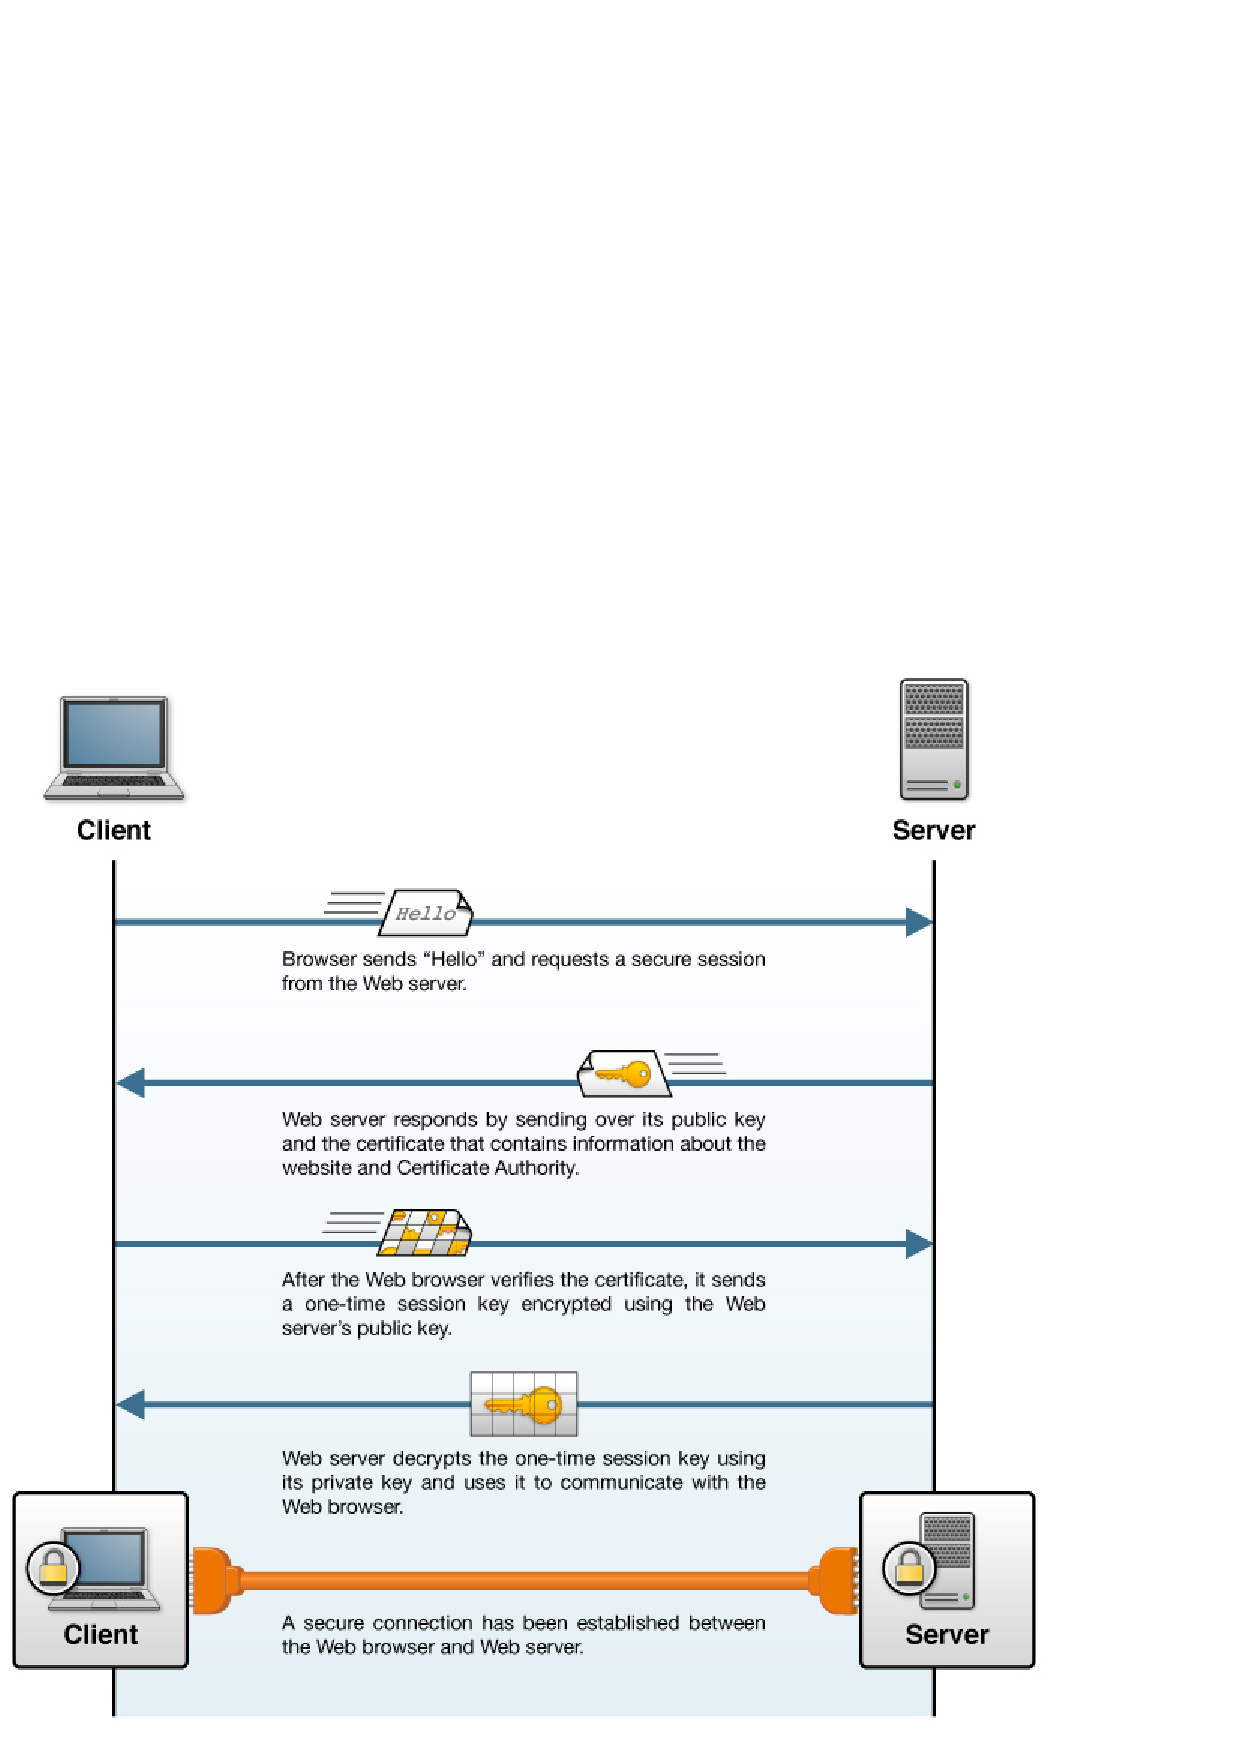
\includegraphics[width=0.5\linewidth]{tls.jpg}
   \caption{TLS Overview\cite{tlsconcepts}}
   \label{fig:tls}
\end{figure}

\subsection{Data Collection}
The proposed protocol given by the RSA actually modeled the certificate model
used by SSL/TLS. For this reason, the SSL certificate model was the primary
focus of the data collected. Moreover, the data set of RSA keys in SSL
certificates is much larger than DRM implementations that use RSA. Thus, the
data set that was collected and then analyzed consisted entirely of X.509
certificates.

Since a primary motivation of this work is the potential impact that vulnerable
RSA keys may have, a data set representative of a large portion of traffic was
desired. A survey was done over 2007-2010 \cite{labovitz2011internet} that
gathered some useful data on the Internet as a whole. Relevant to web traffic,
this study showed that together, the major content data networks (CDN) (i.e.
Google, Facebook, Amazon, etc.) account for nearly 17\% of web traffic.
Specific breakdowns and conversions can be found in Table \ref{tab:traffic}.

\begin{table}
\centering
\caption{Major CDN Traffic (2010)}
\begin{tabular}{|>{\raggedright}p{0.4\linewidth}
                |>{\raggedright}p{0.2\linewidth}
                |>{\raggedright\arraybackslash}p{0.2\linewidth}|}\hline
   \textbf{CDN} & \textbf{Percent of all Internet traffic} & \textbf{Approx. percentage of web traffic}\\ \hline
Google & 7 & 12.72\\ \hline
Facebook & 0.45& 0.818\\ \hline
Amazon CDN (NASA/JPL, PBS,\dots) & 0.55 & 1\\ \hline
EdgeCast (Yahoo!, Break, Imgur,\dots) & 0.5 & 0.909\\ \hline
LeaseWeb (Heineken, Starbucks,\dots) & 0.8 & 1.454\\
\hline\end{tabular}
\label{tab:traffic}
\end{table}

Alexa was used to find websites with large amounts of
traffic\footnote{http://www.alexa.com/}, as it serves as one of the Internet's
most prevalent sources for traffic information. In addition to individualized
site traffic data, Alexa provides a daily-updated list of the top one million
websites ordered by
traffic\footnote{http://s3.amazonaws.com/alexa-static/top-1m.csv.zip}. In
regards to the previous point concerning CDNs and traffic breakdowns, it was
noted that all web sites hosted by the major CDNs from
\cite{labovitz2011internet} are present in the top one million list.
Additionally, the vast majority of sites from the top one million list were
not provided by the CDNs mentioned in \cite{labovitz2011internet}. This means
that a much larger percentage than 17\% is actually represented by the sites
in the list, although quantifying precisely how much becomes difficult, and
lies beyond the scope of this project.

A Python script was used to parse the CSV file provided by Alexa. Each
extracted URL was visited on port 443 (corresponding to ``https://") using 
\texttt{openssl}. If a site responded on that port, it provided an X.509
certificate to be parsed and verified. Most of the time, this is done by a
user's web browser which has certificate authorities' private keys hidden
within. However, since the work here was not concerned with the actual web
content, the certificate was simply saved. When certificates were found, the
``Subject Public Key Algorithm" section was inspected. If this contained some
form of RSA, \texttt{openssl} was used again to extract the RSA key and save
it into a PEM file (a standard format for saving public and private key
information in). Additionally, since part of this work's motivation lies in
expanding the work done in \cite{scharfglass2012breaking}, the keys were also
stored into a SQLite3 database so that later retrieval by the tool was trivial.

After writing an initial implementation of the Python script, it was realized
that the collection process was too slow. Therefore, some of Python's
multi-process capabilities were utilized to speed up the collection of data.
Eight processes were spawned to perform the work described above. Seven of the
processes read URLs from a deque (double-ended queue) and attempted to obtain
an X.509 certificate and RSA key from each. When found, these keys were added
to a queue. These data structures not only offered convenient structures for
organizing the data, but were also thread-safe and could be used with our
updated implementation. An eighth thread read keys from the queue and entered
them into the SQLite3 database. This reimplementation offered a 15$\times$
speedup over the previous, na\"{i}ve approach.

\subsection{Data Analysis}
After collecting data from each of the top one million Alexa sites, some
surface-level analysis was performed in order to gain an overview of the
security of these one million sites. This analysis included overall security
breakdowns (i.e. whether a site used any kind of security) and
bit-length breakdowns of the RSA keys that were found. This data analysis can
be found in Figures \ref{fig:certs} and \ref{fig:bits}. Table \ref{tab:bits}
offer specific breakdown for bit-lengths, and offers details that cannot be
seen in the figure.

\begin{figure}
   \centering
   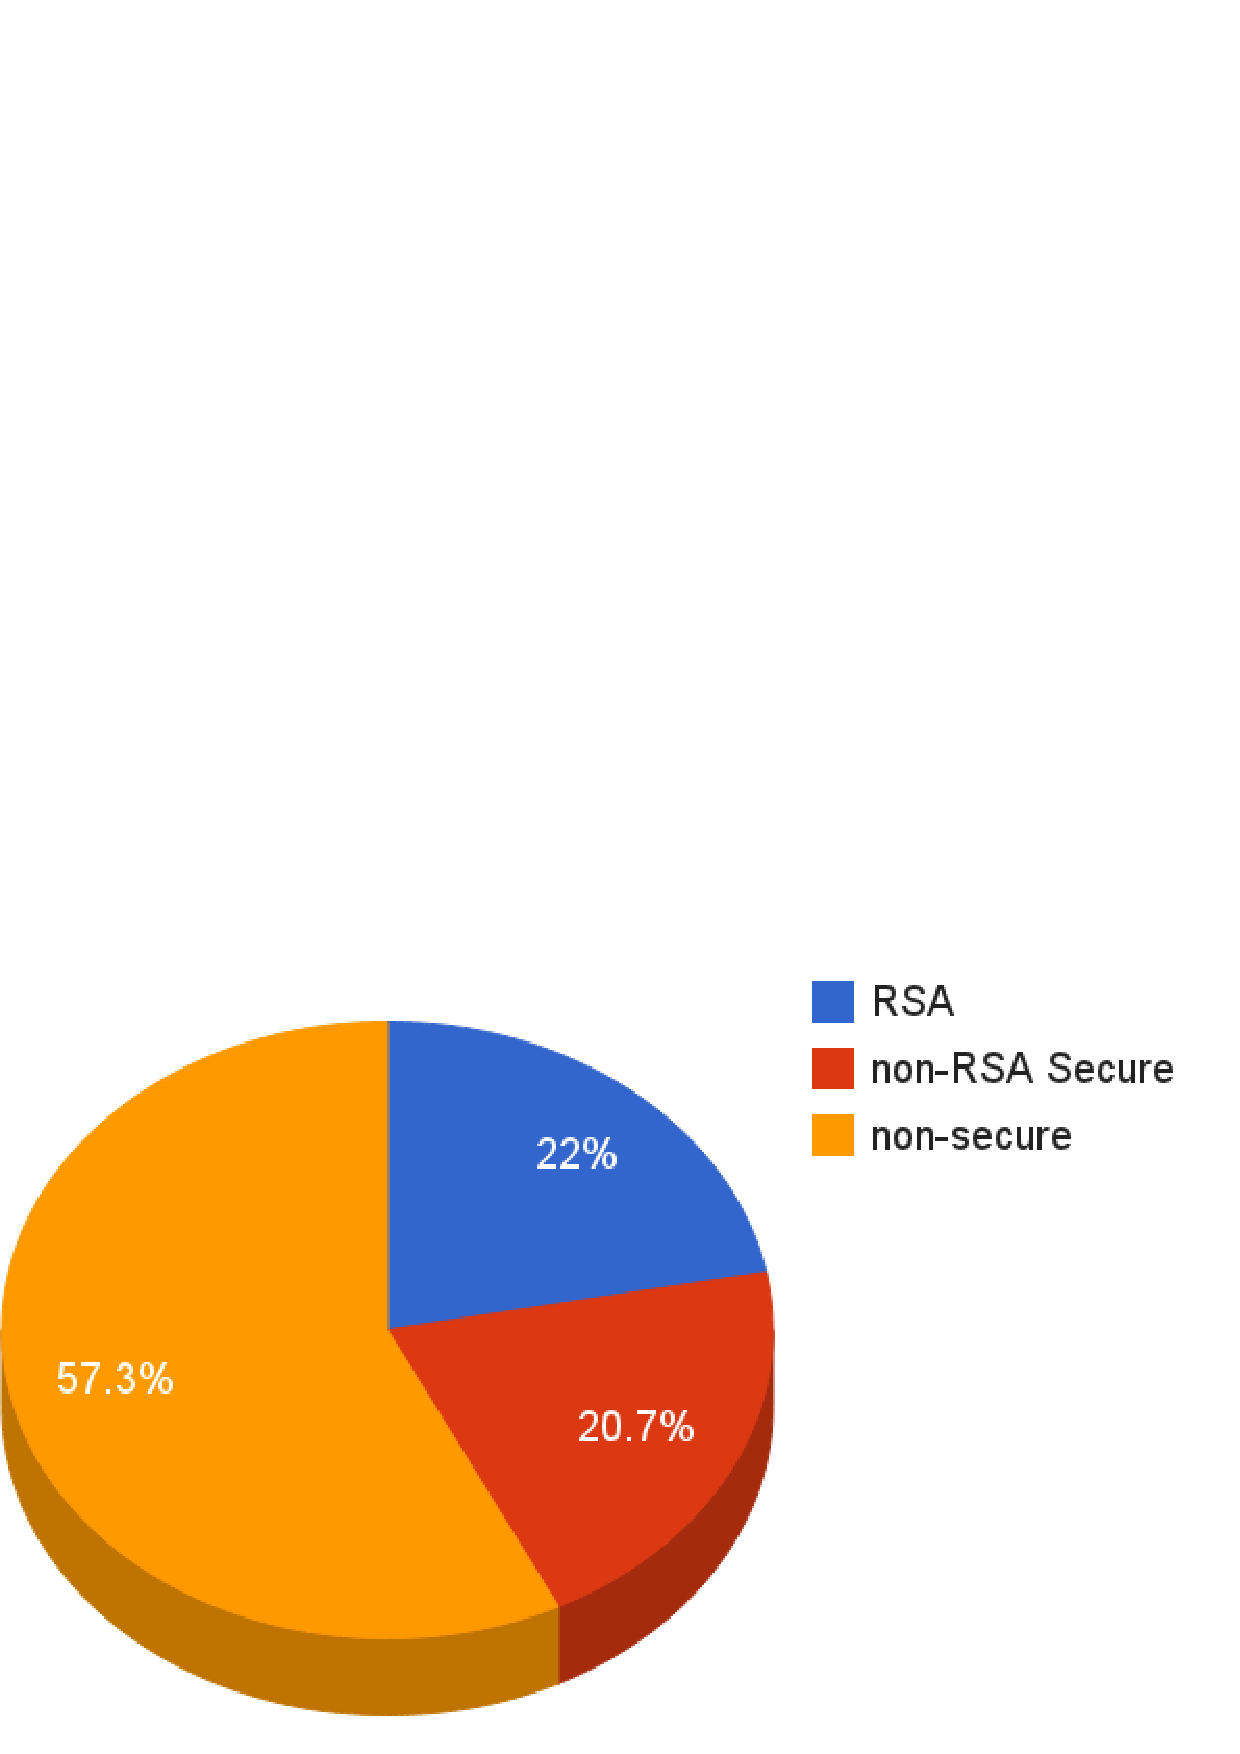
\includegraphics[width=0.75\linewidth]{cert_security.png}
   \caption{Presence of RSA key or other security in Alexa top 1M sites}
   \label{fig:certs}
\end{figure}

Interestingly (and slightly worrisome), is that the majority of web sites in
this top one million list did not even respond on port 443, implying that
they do not allow any option for secure traffic to their site. Nearly 60\% of
websites in the list fell into this category.

Also of note are the specifics of bit-lengths found. It is a surprising data
set for various reasons. First, bit-lengths as small as 384, 512, and 768 were
not expected as keys of this size were factored years ago
\cite{rsa2007challenge}, and cannot be expected to offer much
security\footnote{Interesting note: The author attempted to visit the sites
384-bit keys. Google Chrome did not find a web page on port 443 for any of
the sites.}.

On the other hand, the high number of longer bit-lengths was also surprising,
but comforting. The fact that the vast majority of keys were 2048-bit was not
expected, but means that a large number of high-traffic websites have adequate
(for now) encryption. Moreover, there were quite a number of sites with 4096,
and, even more surprisingly, 8192-bit.

\begin{figure}
   \centering
   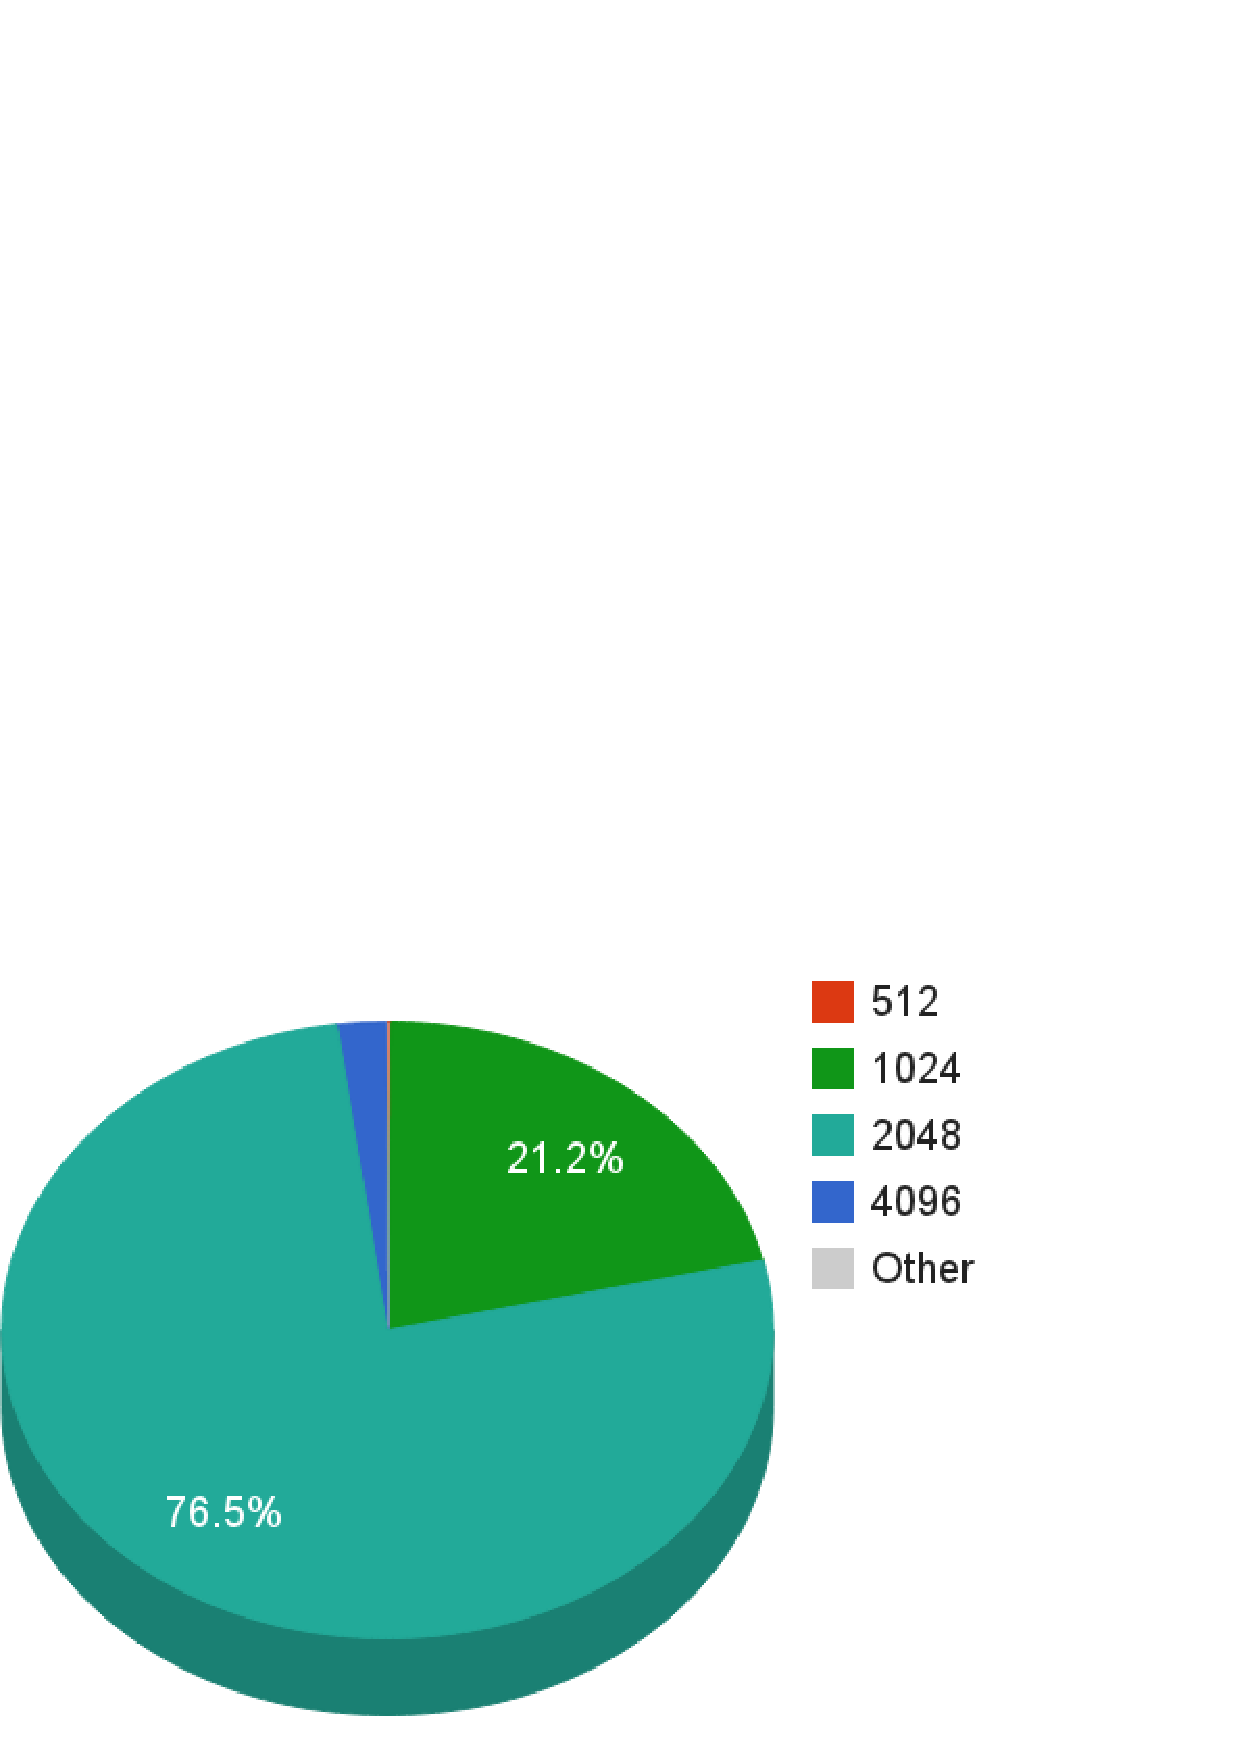
\includegraphics[width=0.75\linewidth]{bit_length.png}
   \caption{Breakdown of Alexa top 1M sites' RSA keys by bit-length}
   \label{fig:bits}
\end{figure}

\begin{table}
\centering
\caption{Alexa top 1M X.509 RSA bit-length}
\begin{tabular}{|r|r|}\hline
\textbf{Bits} & \textbf{Count}\\\hline
384 & 4 \\ \hline
512 & 309 \\ \hline
768 & 4 \\ \hline
1024 & 46736 \\ \hline
2048 & 168391 \\ \hline
2432 & 37 \\ \hline
3072 & 17 \\ \hline
4096 & 4511 \\ \hline
8192 & 14 \\ \hline
other & 44 \\ \hline
\end{tabular}
\label{tab:bits}
\end{table}

Further analysis was done using the tool described in
\cite{scharfglass2012breaking}. This tool performs a complete check of all
RSA keys in a given set for the previously mentioned vulnerability described
in \cite{lenstra2012ron}. This check is done using NVIDIA's CUDA framework to
parallelize the work as much as possible which allows for a practical security
validation tool. At the time of writing, the tool's current implementation is
limited to 1024-bit RSA keys. Due to this limitation, the data set was
reduced to 46,736 RSA keys. Due to the $O(n^2)$ nature of this problem,
this check resulted in $1,092,150,216$ comparisons. The run of the tool using
this data set took 138 minutes, 37 seconds or $131,305$ comparisons per second.
After applying the tool to this set of keys, it was found that no keys were
susceptible to the vulnerability (insofar as none of the keys in the set
shared primes with a given key). Although no vulnerabilities were detected,
this does not mean the set is completely secure from the previously mentioned
vulnerability. Since such a limited data set was used, and the security tool
relies on large sets to accumulate many primes, the analysis presented can
only be considered an initial pass.

\subsection{Implications}
For the same reasons the data set was chosen to be X.509 certificates, presence
of the vulnerability mentioned here would have the largest effect on Internet
security: specifically in the certificate infrastructure. If servers were
unknowingly providing compromised public keys in their certificates, their
traffic could offer no security if this became known. This could offer
ill-effects since the vulnerability is agnostic of the type of data being
being encrypted.

Additionally, the password-alternatives that were mentioned briefly before
could be particularly impacted. If a system was generating many new RSA keys
(e.g. a user is building new accounts for various websites, and tying RSA keys
to them) with inadequate primes, potentially all these accounts for this user
could end up compromised, despite the sense of stronger security.

Along these lines, a system administrator could potentially suffer from similar
issues. If many machines and key-pairs are being setup and generated as part of
an initial setup process for a new network of users, poor random number
generation could have severe consequences when done at scale. This would likely
create many new, vulnerable keys at once. By being aware that this problem
could exist, and that a tool such as \cite{scharfglass2012breaking} exists, an
insecure set of users could be avoided or detected much earlier than would have
otherwise occurred.

% probably unnecessary at this point
%\subsection{Future Work}
%As mentioned, this survey suffers from various limitations. Some immediate
%steps are recommended to make the analysis more complete. Primarily, a larger
%data set of any kind must be used with the tool in
%\cite{scharfglass2012breaking}. This could come in several ways. First,
%additional keys could be generated and added to the set of $46,736$ so that more
%prime values are present in the pool of primes. Second, more primes could be
%collected from other certificates online. The tool gains functionality as the
%number of keys increases, so the more keys used, the more complete the results.
%
%Furthermore, extending the functionality to 2048-bit keys would offer several
%advantages over the present work. First, a much more accurate analysis of
%high-traffic X.509 certificates could be gained since this was the largest
%portion of the data collected (see Figure \ref{fig:bits}). Second, it would
%offer a much larger data set, which, as previously mentioned, adds
%effectiveness to the tool.
%
%The survey could also be expanded to include public keys from the 
%previously-mentioned self-maintained keys (e.g. password alternatives). If
%these keys were accessible from some set of services, it could contribute to
%the data sets significantly. This would especially hold true if there existed
%ways to correlate where specific keys originated form (i.e. which machine
%generated them). This way, when vulnerable keys were found, a machine could be
%flagged as potentially insecure for key generation.
%
\subsection{Conclusions}
This survey determined that the primary use of RSA keys in practice is the
signing of SSL certificates. A data set was gathered that accounts for a
significant amount of certificates in the context of web traffic. Some
surface-level analysis was done to gain a general understanding of the
collected data. A high-performance tool was then applied to a subset of the
data to check for a vulnerability within the data subset. No vulnerabilities
were found; however, due to limitations in the tool used, as well as
limitations in the data set, this cannot be considered a complete analysis
and requires further investigation.

Though limited, this survey does successfully add real-world application
context to the work done in \cite{scharfglass2012breaking}. Specific
implications are able to be draw from the practicality of the tool, and more
tangible examples of what vulnerabilities in RSA keys looks like have been
realized.

%%%%%%%%%%%%%%%%%%%%%%%%%%%%%%%%%%%%%%%%%%%%%%%%%%%%%%%%%%%%%%%%%%%%%%%%%%%%%%%

\chapter{Related Works}
\label{related}

\section{The Vulnerability}
An RSA vulnerability was discovered and detailed in \cite{lenstra2012ron} in
early 2012 that forms the basis of the exploit the work presented here builds
upon. Namely, that poor random number generation in RSA keys results in
insecure encryption using these keys. Specifically, a key's private components
can be generated using publicly available information by taking advantage of
the work presented in \cite{scharfglass2012breaking}.

The exploit explored in \cite{lenstra2012ron} makes use of the two prime
values that play a fundamental role in an RSA key. These values must be
sufficiently random such that repeated values are infeasible and mathematically
extremely improbable to encounter due to the scope of the set (this work
focuses on 1024-bit keys). However, on some systems and due to some
less-than-adequate code, this may not always be the case. When these values are
repeated between keys, the greatest-common-divisor algorithm can be applied to
find the shared value between keys. This is significant because the GCD
calculation is significantly less computationally expensive than the
alternative: factoring the large values. With this new information about each key,
they private components are straight-forward to generate since the RSA
key-generation process is public and not difficult to implement.

A large sample set was obtained via the OpenSSL Observatory and by crawling the
Internet for SSL certificates (which use RSA as an encryption scheme). Since it
was thought this would provide an adequate sample set, all these keys were
analyzed. The set contained 1024-bit keys, as well as 2048-bit keys. The
findings were that 0.2\% of these keys were vulnerable to this exploit, and
thus offered no security. This included 2048-bit keys as well, despite the
conception 2048-bit keys are more secure (this would be true if this
vulnerability were avoided).

\section{The Process}
As mentioned, the vulnerability is exploited by performing greatest common
divisor (GCD) calculations with pairs of keys. The research presented in this
paper looks at how to most quickly and efficiently analyze a large database of
RSA keys and detect if this vulnerability is present within the set.
Traditionally, this would be a tedious process that would likely be infeasible
due to time constraints. Since the calculations are independent of one another
(between pairs of keys) they can be done in parallel, given the proper system.
One such system, and the focus of this work, is NVIDIA's CUDA. This will be
detailed later, however, it relates to work done in \cite{fujimoto2009high}. 

This work optimized a specific version of the GCD (binary GCD). This method
reduces the algorithm to three repeated operations. This algorithm was then
implemented in CUDA for 1024-bit numbers (something CUDA does not offer native
support for). This allows much of each operation to be performed in a parallel
fashion, further optimizing the process.

\section{Completed Areas}
As a groundwork for the research presented here, the work done in
\cite{scharfglass2012breaking} will be used extensively. Here, the ideas present in
both \cite{lenstra2012ron} and \cite{fujimoto2009high} are combined with
further optimization and parallelization of the data to achieve a significant
speedup of the overall process (when compared to the sequential runtimes). This
work makes use of CUDA to parallelize the binary GCD algorithm as presented in
\cite{fujimoto2009high}, but additionally parallelizes each GCD calculation as
each is independent of the other (that is, many complete GCD comparisons are 
performed in parallel). This same approach will be used in the work that follows.

This work, however, does not offer a complete solution and suffers from several
limitations. The work in \cite{scharfglass2012breaking} does not actually produce
the private components of the RSA keys found to be vulnerable by the algorithm.
Furthermore, the set of keys that can be used in the algorithm as presented, is
limited by the memory present on the GPU. To offer a complete solution, this
must be overcome to allow RSA key-sets of arbitrary size to be used for the
validation. The usefulness of such work is severely impacted due to these two
limitations.

\section{Multiple GPUs}
As an extension to the work in \cite{scharfglass2012breaking}, multiple GPU support
will be explored. This concept is discussed at length in
\cite{schaa2009exploring}. Here, several GPU configurations are investigated to
analyze how a distributed system may benefit over a single-GPU design.
Work is divided intelligently among the systems in the distributed system to
gain more performance increase than would be possible with a single system.

At the time \cite{schaa2009exploring} was written, single-system,
multiple-GPU configurations were not possible using CUDA over SLI (Scalable
Link Interface, NVIDIA's brand for the interface between multiple GPUs).
However, this is possible now, and will be explored at length in our work.
This configuration offers benefits including transfer speeds over alternative
configurations.

The work done in \cite{thibault2009cuda} helps to make a case for the
additional speedup that making use of multiple GPUs can offer. This work was
done after CUDA had added adequate support for using multiple GPUs
simultaneously, and configurations with two-GPU and four-GPU systems were used.

Significant additional speedups were gained, ranging up to three times speedup
using four GPUs over the single-GPU system (which translates to 100 times
speedup compared to the original, non-GPU benchmark being used). This kind of
speedup offers great optimism in how multiple GPUs may offer significant
increases to performance of the GCD key algorithm.

Another interesting aspect of the work done in \cite{thibault2009cuda} is the
varied domain sizes that were used. The data sets were broken down into several
different configurations which was each tested on the single, dual, or quad-GPU
configuration. This was done to achieve a more accurate answer to how much
faster the multi-GPU system could be. The largest domain set
($1024\times32\times1024$), interestingly, offered the greatest additional
speedup between configurations---the quad-GPU configuration was 3 times faster
than the single-GPU, compared to 2 times for the $256\times32\times256$
domain. This is significant, and implies that exploring different ways to
organize our own data may offer increased advantages when moving to a multi-GPU
system.

\section{Large Data}
Since one of our primary goals is to remove the limitation present in
\cite{scharfglass2012breaking} that prevents larger sets of keys from being
analyzed, work investigating how to manage large data sets is relevant.
Specifically, large data sets that must be managed by the GPU.

One such work is \cite{wu2009clustering}. In this work, like our own, the data
is too large to fit within the extremely-limited memory of the GPU. Thus, the
data must be partitioned. In this work, the data was first prepared by
organizing it so that it could be effectively partitioned. There was a
straightforward way of doing so for this application (K-means).

Additionally, some features of the GPU were considered and used, namely
asynchronous memory transfer, a type of multi-tasked streaming. This feature
allows memory transfers to be done between the GPU and CPU while the GPU is
processing data it already has. This can increase performance significantly
when compared to having the GPU move from processing to data transfer (i.e.
having a single tasked thread). Optimization of threads was looked into in this
work as well, as the authors attempted to find how many of these threads would
add the positively impact speedup the most. They found that only 2 threads
(i.e. one processing, one transferring) were needed to gain the greatest
performance benefit. Adding additional streams after this point did not offer
additional benefit.

Decomposition of data is the primary problem when attempting to perform work
with a GPU due to the limitations of current hardware. Therefore, much work and
thought has been given to optimizing the structure of large data sets. Although
a different type of parallelism is looked at in \cite{charles2012chunking}, the
strategies to data decomposition are relevant to most parallel problem in
general, including CUDA. The focus in this survey is matrix multiplication,
a standard parallel problem. The most effective way to chunk the data in this
work appears to be entire rows/columns of the element matrices. This is logical,
and the approach is mimicked (as much as it can be since matrix multiplication
is not perfectly synonymous) in \cite{scharfglass2012breaking}. However, a slight
modification was found to make this strategy most effective: hold the results
in memory until an entire set of iterations completes (all that will fit in
memory) and only then transfer the results back to the CPU. Although this does
not decrease the amount of memory sent from the GPU to the CPU, it reduces the
number of total memory transfers which is often more important. Such fine
details must be found and applied to our work here to further increase our
performance.

\section{Optimization}
As mentioned, data decomposition and organization around the architecture are
some of the most important (if not \emph{the} most important) aspects of
creating a parallel solution for use with a GPGPU. The work done in
\cite{ryoo2008optimization} gives a detailed overview of how one might optimize
work done with CUDA. It discusses the memory model, and how certain techniques
such as tiling are used to optimize the performance gains. Although some of
these techniques are used in the original implementation found in
\cite{scharfglass2012breaking}, it does not appear that they were used extensively.
It seems that the research and surveying done in \cite{ryoo2008optimization}
can be applied to our work here and our speedup will benefit from their results.

Unfortunately, this work was done before multi-GPU systems were fully available
and accessible using CUDA. The optimization strategies presented in this work
will no doubt be useful; however, other strategies also must be employed that
considered systems with more than a single GPU (such as those mentioned here
from \cite{thibault2009cuda}). Leveraging techniques in both realms will offer
the greatest amount of performance gain.

\section{Similar Algorithms}
A similar algorithm that suffers from the same problems that pairwise
comparisons does (each element much be traversed and compared), is search. The
work done in \cite{peters2011fast} explores how search can be optimized for the
CUDA framework. Two approaches are given to the bitonic search algorithm that
is used: the initial, most straight-forward implementation, and another
implementation optimized around the CUDA memory model. The latter offered
significant performance increases over the original. 

A similar approach will be applied to the work that is used from
\cite{scharfglass2012breaking}. Namely, shared memory will be used as efficiently
as possible to allow CUDA to perform at its greatest capacity. This is a vital
concept in general when optimizing for CUDA; however, the work and challenges
from \cite{peters2011fast} are similar to our own, so the implementation
overlaps more than arbitrary examples.

Another important contribution to the field and concepts of distributed systems
is the work presented in \cite{dean2008mapreduce}. MapReduce has become an
extremely useful tool for companies like Google with massive data centers that
must distribute the work to perform as reasonable (real-time) levels. MapReduce
explores how work might be delegated to multiple workers that exist in a
particular distributed system. These concepts apply to the problem of
performing the necessary GCD comparisons using multiple GPUs in a single
system.

%%%%%%%%%%%%%%%%%%%%%%%%%%%%%%%%%%%%%%%%%%%%%%%%%%%%%%%%%%%%%%%%%%%%%%%%%%%%%%%

\chapter{Validation}
Accuracy and speedup will both be validated to gain a measure of success.

To validate accuracy, a sequential implementation will be compared against.
Much as the work found in \cite{scharfglass2012breaking} performed accuracy
validation, a separate, sequential implementation will be created and ran
alongside the parallel implementation. Since this work will function as an
extension to \cite{scharfglass2012breaking}, the validation process will likely be
identical or even reused. The results each implementation produces must match
for a given set of keys (i.e. both implementations must find the same set of
vulnerable keys given identical sets to start with).

An additional limitation realized in \cite{scharfglass2012breaking} was the runtime
of the sequential version becoming too long for large sets of keys. Since this
is known to be an extremely time-consuming process, it will not always be
performed with larger sets of keys. If correct operation of the parallel
implementation for small (i.e. sets that can be run sequential in a reasonable
amount of time) can be validated using many varying sets of keys of increasing
number, it can be assumed the same level of accuracy will continue for larger
sets that will not be run sequentially. Thus, accuracy will be validated for
sets no larger than 200,000 keys (as in \cite{scharfglass2012breaking}), and
assumed to be accurate (given success of the aforementioned validation) for
sets larger than this.

Speedup validation also involves comparing with a sequential implementation;
however, this time the runtimes will be compared so an overall speedup may be
calculated. Again, much as in \cite{scharfglass2012breaking}, speedup will be
calculated by taking the ratio of the sequential and parallel runtimes.

As seen in \cite{scharfglass2012breaking}, the speedup reached an upper threshold,
namely, 27.5. Since this work will expand upon on that, it seems natural to use
27.5 as a baseline. However, there are some differences to consider. First,
in \cite{scharfglass2012breaking}, sets of keys that could fit entirely in the
GPU's memory were tested and presented. This ensures that the number of memory
transfers to the memory card is 1: this significantly reduces memory transfer
time, and would help increase the speedup. Since one goal of this work is to
allow an arbitrary number of keys to be used in a set, this will likely affect
the overall speedup since memory transfers will become smaller and more
frequent.

On the other hand, another goal is to add multi-card support which would
further increase the total speedup of the final, parallel implementation. Since
we will be looking at how fast additional cards make the process (compared to
the single-card implementation), the sequential runtime will become less
important. It will continue to serve as a baseline to the entire algorithm
though. 

Considering the modifications done, speedup near 25 seems like a reasonable
expectation. Functionality that is expected to decrease the original 27.5, as
well as additions that are expected to increase it will both be researched and
added. Therefore, a speedup in the same area appears to be a fair expectation
of success.

% ------------- End main chapters ----------------------

\clearpage
\bibliographystyle{abbrv}
\bibliography{references}

\end{document}
